\section{Gravitational Waveform Catalog}
\label{app:gw_waveform_catalog}

The following figures show the extracted \(r\Psi_4^{(2,2)}\) waveforms at
\(r\simeq 100M\). For each mass ratio and spin, the neutral case is shown
above the charged configurations. The charged cases are ordered by charge
magnitude and charge configuration.

% Compact waveform panel macro.
% This version is compatible with \usepackage[caption=false]{subfig}.
\newcommand{\gwpanel}[1]{%
    \subfloat[]{%
        \includegraphics[width=0.315\textwidth]{#1}%
    }%
}

\newcommand{\gwneutralpanel}[1]{%
    \subfloat[]{%
        \includegraphics[width=0.315\textwidth]{#1}%
    }%
}

% ============================================================
% q = 1, chi = 0
% ============================================================
\begin{figure}[p]
\centering

\gwneutralpanel{Waveform/GW/Q1_SPIN_0_Q0_emda_prof_GW_l2_m2_r5.pdf}

\vspace{0.6em}

\gwpanel{Waveform/GW/Q1_SPIN_0_Q0p05_p0_emda_prof_GW_l2_m2_r5.pdf}
\hfill
\gwpanel{Waveform/GW/Q1_SPIN_0_Q0p05_pn_emda_prof_GW_l2_m2_r5.pdf}
\hfill
\gwpanel{Waveform/GW/Q1_SPIN_0_Q0p05_pp_emda_prof_GW_l2_m2_r5.pdf}

\vspace{0.6em}

\gwpanel{Waveform/GW/Q1_SPIN_0_Q0p1_p0_emda_prof_GW_l2_m2_r5.pdf}
\hfill
\gwpanel{Waveform/GW/Q1_SPIN_0_Q0p1_pn_emda_prof_GW_l2_m2_r5.pdf}
\hfill
\gwpanel{Waveform/GW/Q1_SPIN_0_Q0p1_pp_emda_prof_GW_l2_m2_r5.pdf}

\vspace{0.6em}

\gwpanel{Waveform/GW/Q1_SPIN_0_Q0p15_p0_emda_prof_GW_l2_m2_r5.pdf}
\hfill
\gwpanel{Waveform/GW/Q1_SPIN_0_Q0p15_pn_emda_prof_GW_l2_m2_r5.pdf}
\hfill
\gwpanel{Waveform/GW/Q1_SPIN_0_Q0p15_pp_emda_prof_GW_l2_m2_r5.pdf}

\caption{Extracted \(r\Psi_4^{(2,2)}\) waveforms for \(q=1\) and \(\chi=0\). The neutral case is shown at the top, followed by charged configurations ordered by increasing charge magnitude and charge configuration.}
\label{fig:gw_catalog_q1_chi0}
\end{figure}

% ============================================================
% q = 1, chi = 0.4
% ============================================================
\begin{figure}[p]
\centering

\gwneutralpanel{Waveform/GW/Q1_SPIN_04_Q0_emda_prof_GW_l2_m2_r5.pdf}

\vspace{0.6em}

\gwpanel{Waveform/GW/Q1_SPIN_04_Q0p05_p0_emda_prof_GW_l2_m2_r5.pdf}
\hfill
\gwpanel{Waveform/GW/Q1_SPIN_04_Q0p05_pn_emda_prof_GW_l2_m2_r5.pdf}
\hfill
\gwpanel{Waveform/GW/Q1_SPIN_04_Q0p05_pp_emda_prof_GW_l2_m2_r5.pdf}

\vspace{0.6em}

\gwpanel{Waveform/GW/Q1_SPIN_04_Q0p1_p0_emda_prof_GW_l2_m2_r5.pdf}
\hfill
\gwpanel{Waveform/GW/Q1_SPIN_04_Q0p1_pn_emda_prof_GW_l2_m2_r5.pdf}
\hfill
\gwpanel{Waveform/GW/Q1_SPIN_04_Q0p1_pp_emda_prof_GW_l2_m2_r5.pdf}

\vspace{0.6em}

\gwpanel{Waveform/GW/Q1_SPIN_04_Q0p15_p0_emda_prof_GW_l2_m2_r5.pdf}
\hfill
\gwpanel{Waveform/GW/Q1_SPIN_04_Q0p15_pn_emda_prof_GW_l2_m2_r5.pdf}
\hfill
\gwpanel{Waveform/GW/Q1_SPIN_04_Q0p15_pp_emda_prof_GW_l2_m2_r5.pdf}

\caption{Extracted \(r\Psi_4^{(2,2)}\) waveforms for \(q=1\) and \(\chi=0.4\). The neutral case is shown at the top, followed by charged configurations ordered by increasing charge magnitude and charge configuration.}
\label{fig:gw_catalog_q1_chi04}
\end{figure}

% ============================================================
% q = 1, chi = 0.8
% ============================================================
\begin{figure}[p]
\centering

\gwneutralpanel{Waveform/GW/Q1_SPIN_08_Q0_emda_prof_GW_l2_m2_r5.pdf}

\vspace{0.6em}

\gwpanel{Waveform/GW/Q1_SPIN_08_Q0p05_p0_emda_prof_GW_l2_m2_r5.pdf}
\hfill
\gwpanel{Waveform/GW/Q1_SPIN_08_Q0p05_pn_emda_prof_GW_l2_m2_r5.pdf}
\hfill
\gwpanel{Waveform/GW/Q1_SPIN_08_Q0p05_pp_emda_prof_GW_l2_m2_r5.pdf}

\vspace{0.6em}

\gwpanel{Waveform/GW/Q1_SPIN_08_Q0p1_p0_emda_prof_GW_l2_m2_r5.pdf}
\hfill
\gwpanel{Waveform/GW/Q1_SPIN_08_Q0p1_pn_emda_prof_GW_l2_m2_r5.pdf}
\hfill
\gwpanel{Waveform/GW/Q1_SPIN_08_Q0p1_pp_emda_prof_GW_l2_m2_r5.pdf}

\vspace{0.6em}

\gwpanel{Waveform/GW/Q1_SPIN_08_Q0p15_p0_emda_prof_GW_l2_m2_r5.pdf}
\hfill
\gwpanel{Waveform/GW/Q1_SPIN_08_Q0p15_pn_emda_prof_GW_l2_m2_r5.pdf}
\hfill
\gwpanel{Waveform/GW/Q1_SPIN_08_Q0p15_pp_emda_prof_GW_l2_m2_r5.pdf}

\caption{Extracted \(r\Psi_4^{(2,2)}\) waveforms for \(q=1\) and \(\chi=0.8\). The neutral case is shown at the top, followed by charged configurations ordered by increasing charge magnitude and charge configuration.}
\label{fig:gw_catalog_q1_chi08}
\end{figure}

% ============================================================
% q = 2, chi = 0
% ============================================================
\begin{figure}[p]
\centering

\gwneutralpanel{Waveform/GW/Q2_SPIN_0_Q0_emda_prof_GW_l2_m2_r5.pdf}

\vspace{0.6em}

\gwpanel{Waveform/GW/Q2_SPIN_0_Q0p05_p0_emda_prof_GW_l2_m2_r5.pdf}
\hfill
\gwpanel{Waveform/GW/Q2_SPIN_0_Q0p05_pn_emda_prof_GW_l2_m2_r5.pdf}
\hfill
\gwpanel{Waveform/GW/Q2_SPIN_0_Q0p05_pp_emda_prof_GW_l2_m2_r5.pdf}

\vspace{0.6em}

\gwpanel{Waveform/GW/Q2_SPIN_0_Q0p15_p0_emda_prof_GW_l2_m2_r5.pdf}
\hfill
\gwpanel{Waveform/GW/Q2_SPIN_0_Q0p15_pn_emda_prof_GW_l2_m2_r5.pdf}
\hfill
\gwpanel{Waveform/GW/Q2_SPIN_0_Q0p15_pp_emda_prof_GW_l2_m2_r5.pdf}

\caption{Extracted \(r\Psi_4^{(2,2)}\) waveforms for \(q=2\) and \(\chi=0\). The neutral case is shown at the top, followed by charged configurations ordered by increasing charge magnitude and charge configuration.}
\label{fig:gw_catalog_q2_chi0}
\end{figure}

% ============================================================
% q = 2, chi = 0.4
% ============================================================
\begin{figure}[p]
\centering

\gwneutralpanel{Waveform/GW/Q2_SPIN_04_Q0_emda_prof_GW_l2_m2_r5.pdf}

\vspace{0.6em}

\gwpanel{Waveform/GW/Q2_SPIN_04_Q0p05_p0_emda_prof_GW_l2_m2_r5.pdf}
\hfill
\gwpanel{Waveform/GW/Q2_SPIN_04_Q0p05_pn_emda_prof_GW_l2_m2_r5.pdf}
\hfill
\gwpanel{Waveform/GW/Q2_SPIN_04_Q0p05_pp_emda_prof_GW_l2_m2_r5.pdf}

\vspace{0.6em}

\gwpanel{Waveform/GW/Q2_SPIN_04_Q0p15_p0_emda_prof_GW_l2_m2_r5.pdf}
\hfill
\gwpanel{Waveform/GW/Q2_SPIN_04_Q0p15_pn_emda_prof_GW_l2_m2_r5.pdf}
\hfill
\gwpanel{Waveform/GW/Q2_SPIN_04_Q0p15_pp_emda_prof_GW_l2_m2_r5.pdf}

\caption{Extracted \(r\Psi_4^{(2,2)}\) waveforms for \(q=2\) and \(\chi=0.4\). The neutral case is shown at the top, followed by charged configurations ordered by increasing charge magnitude and charge configuration.}
\label{fig:gw_catalog_q2_chi04}
\end{figure}

% ============================================================
% q = 4, chi = 0.4
% ============================================================
\begin{figure}[p]
\centering

\gwneutralpanel{Waveform/GW/Q4_SPIN_04_Q0_emda_prof_GW_l2_m2_r5.pdf}

\vspace{0.6em}

\gwpanel{Waveform/GW/Q4_SPIN_04_Q0p05_p0_emda_prof_GW_l2_m2_r5.pdf}
\hfill
\gwpanel{Waveform/GW/Q4_SPIN_04_Q0p05_pn_emda_prof_GW_l2_m2_r5.pdf}
\hfill
\gwpanel{Waveform/GW/Q4_SPIN_04_Q0p05_pp_emda_prof_GW_l2_m2_r5.pdf}

\caption{Extracted \(r\Psi_4^{(2,2)}\) waveforms for \(q=4\) and \(\chi=0.4\). The neutral case is shown at the top, followed by the charged configurations.}
\label{fig:gw_catalog_q4_chi04}
\end{figure}

% ============================================================
% q = 8, chi = 0.2
% ============================================================
\begin{figure}[p]
\centering

\subfloat[Neutral configuration.]{%
    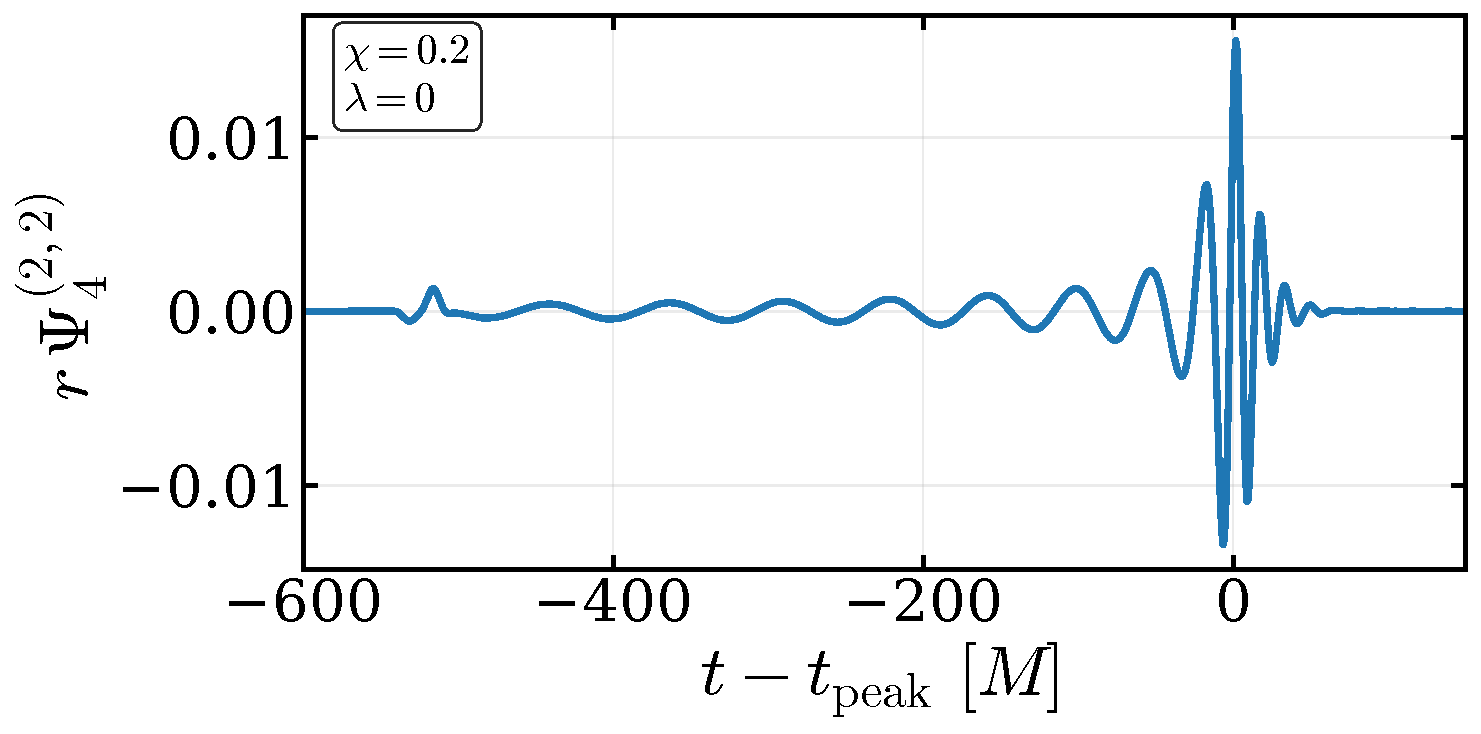
\includegraphics[width=0.47\textwidth]{Waveform/GW/Q8_SPIN_02_Q0_emda_prof_GW_l2_m2_r5.pdf}%
}
\hfill
\subfloat[Charged \(++\) configuration.]{%
    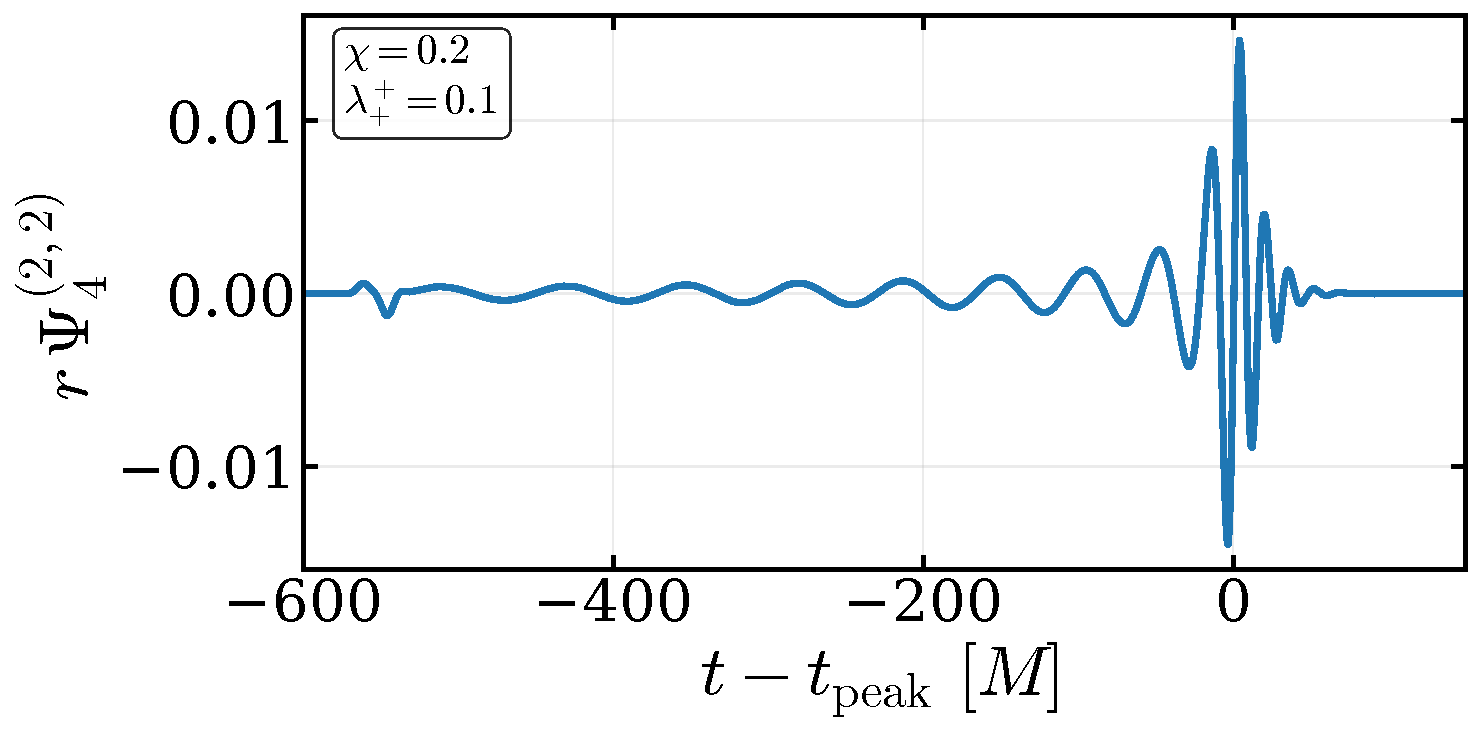
\includegraphics[width=0.47\textwidth]{Waveform/GW/Q8_SPIN_02_Q0p1_pp_emda_prof_GW_l2_m2_r5.pdf}%
}

\caption{Extracted \(r\Psi_4^{(2,2)}\) waveforms for \(q=8\) and \(\chi=0.2\).}
\label{fig:gw_catalog_q8_chi02}
\end{figure}

% ============================================================
% Scalar waveform catalog macros
% Compatible with \usepackage[caption=false]{subfig}
% ============================================================

\newcommand{\fieldpanel}[2]{%
    \subfloat[#1]{%
        \includegraphics[width=0.315\textwidth]{#2}%
    }%
}

% ============================================================
% PHI1 waveform catalog
% ============================================================
\section{\texorpdfstring{\(\Phi_1\)}{Phi1} Waveform Catalog}
\label{app:phi1_waveform_catalog}

The following figures show the extracted \(\Phi_1\) waveforms at
\(r\simeq 100M\). Since there is no radiation in the neutral case,
only charged configurations are shown. The charged cases are ordered
by charge magnitude and charge configuration. For the \(+-\) cases,
we show the \((\ell,m)=(1,1)\) mode, while for the \(+0\) and \(++\)
cases we show the \((\ell,m)=(2,2)\) mode.

% ============================================================
% PHI1: q = 1, chi = 0
% ============================================================
\begin{figure}[p]
\centering

\fieldpanel{\(Q0p05,+0\)}
{Waveform/PHI1/Q1_SPIN_0_Q0p05_p0_emda_prof_PHI1_l2_m2_r5.pdf}
\hfill
\fieldpanel{\(Q0p05,+-\)}
{Waveform/PHI1/Q1_SPIN_0_Q0p05_pn_emda_prof_PHI1_l1_m1_r5.pdf}
\hfill
\fieldpanel{\(Q0p05,++\)}
{Waveform/PHI1/Q1_SPIN_0_Q0p05_pp_emda_prof_PHI1_l2_m2_r5.pdf}

\vspace{0.6em}

\fieldpanel{\(Q0p1,+0\)}
{Waveform/PHI1/Q1_SPIN_0_Q0p1_p0_emda_prof_PHI1_l2_m2_r5.pdf}
\hfill
\fieldpanel{\(Q0p1,+-\)}
{Waveform/PHI1/Q1_SPIN_0_Q0p1_pn_emda_prof_PHI1_l1_m1_r5.pdf}
\hfill
\fieldpanel{\(Q0p1,++\)}
{Waveform/PHI1/Q1_SPIN_0_Q0p1_pp_emda_prof_PHI1_l2_m2_r5.pdf}

\vspace{0.6em}

\fieldpanel{\(Q0p15,+0\)}
{Waveform/PHI1/Q1_SPIN_0_Q0p15_p0_emda_prof_PHI1_l2_m2_r5.pdf}
\hfill
\fieldpanel{\(Q0p15,+-\)}
{Waveform/PHI1/Q1_SPIN_0_Q0p15_pn_emda_prof_PHI1_l1_m1_r5.pdf}
\hfill
\fieldpanel{\(Q0p15,++\)}
{Waveform/PHI1/Q1_SPIN_0_Q0p15_pp_emda_prof_PHI1_l2_m2_r5.pdf}

\caption{Extracted \(\Phi_1\) waveforms for \(q=1\) and \(\chi=0\).}
\label{fig:phi1_catalog_q1_chi0}
\end{figure}

% ============================================================
% PHI1: q = 1, chi = 0.4
% ============================================================
\begin{figure}[p]
\centering

\fieldpanel{\(Q0p05,+0\)}
{Waveform/PHI1/Q1_SPIN_04_Q0p05_p0_emda_prof_PHI1_l2_m2_r5.pdf}
\hfill
\fieldpanel{\(Q0p05,+-\)}
{Waveform/PHI1/Q1_SPIN_04_Q0p05_pn_emda_prof_PHI1_l1_m1_r5.pdf}
\hfill
\fieldpanel{\(Q0p05,++\)}
{Waveform/PHI1/Q1_SPIN_04_Q0p05_pp_emda_prof_PHI1_l2_m2_r5.pdf}

\vspace{0.6em}

\fieldpanel{\(Q0p1,+0\)}
{Waveform/PHI1/Q1_SPIN_04_Q0p1_p0_emda_prof_PHI1_l2_m2_r5.pdf}
\hfill
\fieldpanel{\(Q0p1,+-\)}
{Waveform/PHI1/Q1_SPIN_04_Q0p1_pn_emda_prof_PHI1_l1_m1_r5.pdf}
\hfill
\fieldpanel{\(Q0p1,++\)}
{Waveform/PHI1/Q1_SPIN_04_Q0p1_pp_emda_prof_PHI1_l2_m2_r5.pdf}

\vspace{0.6em}

\fieldpanel{\(Q0p15,+0\)}
{Waveform/PHI1/Q1_SPIN_04_Q0p15_p0_emda_prof_PHI1_l2_m2_r5.pdf}
\hfill
\fieldpanel{\(Q0p15,+-\)}
{Waveform/PHI1/Q1_SPIN_04_Q0p15_pn_emda_prof_PHI1_l1_m1_r5.pdf}
\hfill
\fieldpanel{\(Q0p15,++\)}
{Waveform/PHI1/Q1_SPIN_04_Q0p15_pp_emda_prof_PHI1_l2_m2_r5.pdf}

\caption{Extracted \(\Phi_1\) waveforms for \(q=1\) and \(\chi=0.4\).}
\label{fig:phi1_catalog_q1_chi04}
\end{figure}

% ============================================================
% PHI1: q = 1, chi = 0.8
% ============================================================
\begin{figure}[p]
\centering

\fieldpanel{\(Q0p05,+0\)}
{Waveform/PHI1/Q1_SPIN_08_Q0p05_p0_emda_prof_PHI1_l2_m2_r5.pdf}
\hfill
\fieldpanel{\(Q0p05,+-\)}
{Waveform/PHI1/Q1_SPIN_08_Q0p05_pn_emda_prof_PHI1_l1_m1_r5.pdf}
\hfill
\fieldpanel{\(Q0p05,++\)}
{Waveform/PHI1/Q1_SPIN_08_Q0p05_pp_emda_prof_PHI1_l2_m2_r5.pdf}

\vspace{0.6em}

\fieldpanel{\(Q0p1,+0\)}
{Waveform/PHI1/Q1_SPIN_08_Q0p1_p0_emda_prof_PHI1_l2_m2_r5.pdf}
\hfill
\fieldpanel{\(Q0p1,+-\)}
{Waveform/PHI1/Q1_SPIN_08_Q0p1_pn_emda_prof_PHI1_l1_m1_r5.pdf}
\hfill
\fieldpanel{\(Q0p1,++\)}
{Waveform/PHI1/Q1_SPIN_08_Q0p1_pp_emda_prof_PHI1_l2_m2_r5.pdf}

\vspace{0.6em}

\fieldpanel{\(Q0p15,+0\)}
{Waveform/PHI1/Q1_SPIN_08_Q0p15_p0_emda_prof_PHI1_l2_m2_r5.pdf}
\hfill
\fieldpanel{\(Q0p15,+-\)}
{Waveform/PHI1/Q1_SPIN_08_Q0p15_pn_emda_prof_PHI1_l1_m1_r5.pdf}
\hfill
\fieldpanel{\(Q0p15,++\)}
{Waveform/PHI1/Q1_SPIN_08_Q0p15_pp_emda_prof_PHI1_l2_m2_r5.pdf}

\caption{Extracted \(\Phi_1\) waveforms for \(q=1\) and \(\chi=0.8\).}
\label{fig:phi1_catalog_q1_chi08}
\end{figure}

% ============================================================
% PHI1: q = 2, chi = 0
% ============================================================
\begin{figure}[p]
\centering

\fieldpanel{\(Q0p05,+0\)}
{Waveform/PHI1/Q2_SPIN_0_Q0p05_p0_emda_prof_PHI1_l2_m2_r5.pdf}
\hfill
\fieldpanel{\(Q0p05,+-\)}
{Waveform/PHI1/Q2_SPIN_0_Q0p05_pn_emda_prof_PHI1_l1_m1_r5.pdf}
\hfill
\fieldpanel{\(Q0p05,++\)}
{Waveform/PHI1/Q2_SPIN_0_Q0p05_pp_emda_prof_PHI1_l2_m2_r5.pdf}

\vspace{0.6em}

\fieldpanel{\(Q0p15,+0\)}
{Waveform/PHI1/Q2_SPIN_0_Q0p15_p0_emda_prof_PHI1_l2_m2_r5.pdf}
\hfill
\fieldpanel{\(Q0p15,+-\)}
{Waveform/PHI1/Q2_SPIN_0_Q0p15_pn_emda_prof_PHI1_l1_m1_r5.pdf}
\hfill
\fieldpanel{\(Q0p15,++\)}
{Waveform/PHI1/Q2_SPIN_0_Q0p15_pp_emda_prof_PHI1_l2_m2_r5.pdf}

\caption{Extracted \(\Phi_1\) waveforms for \(q=2\) and \(\chi=0\).}
\label{fig:phi1_catalog_q2_chi0}
\end{figure}

% ============================================================
% PHI1: q = 2, chi = 0.4
% ============================================================
\begin{figure}[p]
\centering

\fieldpanel{\(Q0p05,+0\)}
{Waveform/PHI1/Q2_SPIN_04_Q0p05_p0_emda_prof_PHI1_l2_m2_r5.pdf}
\hfill
\fieldpanel{\(Q0p05,+-\)}
{Waveform/PHI1/Q2_SPIN_04_Q0p05_pn_emda_prof_PHI1_l1_m1_r5.pdf}
\hfill
\fieldpanel{\(Q0p05,++\)}
{Waveform/PHI1/Q2_SPIN_04_Q0p05_pp_emda_prof_PHI1_l2_m2_r5.pdf}

\vspace{0.6em}

\fieldpanel{\(Q0p15,+0\)}
{Waveform/PHI1/Q2_SPIN_04_Q0p15_p0_emda_prof_PHI1_l2_m2_r5.pdf}
\hfill
\fieldpanel{\(Q0p15,+-\)}
{Waveform/PHI1/Q2_SPIN_04_Q0p15_pn_emda_prof_PHI1_l1_m1_r5.pdf}
\hfill
\fieldpanel{\(Q0p15,++\)}
{Waveform/PHI1/Q2_SPIN_04_Q0p15_pp_emda_prof_PHI1_l2_m2_r5.pdf}

\caption{Extracted \(\Phi_1\) waveforms for \(q=2\) and \(\chi=0.4\).}
\label{fig:phi1_catalog_q2_chi04}
\end{figure}

% ============================================================
% PHI1: q = 4, chi = 0.4
% ============================================================
\begin{figure}[p]
\centering

\fieldpanel{\(Q0p05,+0\)}
{Waveform/PHI1/Q4_SPIN_04_Q0p05_p0_emda_prof_PHI1_l2_m2_r5.pdf}
\hfill
\fieldpanel{\(Q0p05,+-\)}
{Waveform/PHI1/Q4_SPIN_04_Q0p05_pn_emda_prof_PHI1_l1_m1_r5.pdf}
\hfill
\fieldpanel{\(Q0p05,++\)}
{Waveform/PHI1/Q4_SPIN_04_Q0p05_pp_emda_prof_PHI1_l2_m2_r5.pdf}

\caption{Extracted \(\Phi_1\) waveforms for \(q=4\) and \(\chi=0.4\).}
\label{fig:phi1_catalog_q4_chi04}
\end{figure}

% ============================================================
% PHI1: q = 8, chi = 0.2
% ============================================================
\begin{figure}[p]
\centering

\fieldpanel{\(Q0p1,++\)}
{Waveform/PHI1/Q8_SPIN_02_Q0p1_pp_emda_prof_PHI1_l2_m2_r5.pdf}

\caption{Extracted \(\Phi_1\) waveforms for \(q=8\) and \(\chi=0.2\).}
\label{fig:phi1_catalog_q8_chi02}
\end{figure}


% ============================================================
% PHI2 waveform catalog
% ============================================================
\section{\texorpdfstring{\(\Phi_2\)}{Phi2} Waveform Catalog}
\label{app:phi2_waveform_catalog}

The following figures show the extracted \(\Phi_2\) waveforms at
\(r\simeq 100M\). Since there is no radiation in the neutral case,
only charged configurations are shown. The charged cases are ordered
by charge magnitude and charge configuration. For the \(+-\) cases,
we show the \((\ell,m)=(1,1)\) mode, while for the \(+0\) and \(++\)
cases we show the \((\ell,m)=(2,2)\) mode.

% ============================================================
% PHI2: q = 1, chi = 0
% ============================================================
\begin{figure}[p]
\centering

\fieldpanel{\(Q0p05,+0\)}
{Waveform/PHI2/Q1_SPIN_0_Q0p05_p0_emda_prof_PHI2_l2_m2_r5.pdf}
\hfill
\fieldpanel{\(Q0p05,+-\)}
{Waveform/PHI2/Q1_SPIN_0_Q0p05_pn_emda_prof_PHI2_l1_m1_r5.pdf}
\hfill
\fieldpanel{\(Q0p05,++\)}
{Waveform/PHI2/Q1_SPIN_0_Q0p05_pp_emda_prof_PHI2_l2_m2_r5.pdf}

\vspace{0.6em}

\fieldpanel{\(Q0p1,+0\)}
{Waveform/PHI2/Q1_SPIN_0_Q0p1_p0_emda_prof_PHI2_l2_m2_r5.pdf}
\hfill
\fieldpanel{\(Q0p1,+-\)}
{Waveform/PHI2/Q1_SPIN_0_Q0p1_pn_emda_prof_PHI2_l1_m1_r5.pdf}
\hfill
\fieldpanel{\(Q0p1,++\)}
{Waveform/PHI2/Q1_SPIN_0_Q0p1_pp_emda_prof_PHI2_l2_m2_r5.pdf}

\vspace{0.6em}

\fieldpanel{\(Q0p15,+0\)}
{Waveform/PHI2/Q1_SPIN_0_Q0p15_p0_emda_prof_PHI2_l2_m2_r5.pdf}
\hfill
\fieldpanel{\(Q0p15,+-\)}
{Waveform/PHI2/Q1_SPIN_0_Q0p15_pn_emda_prof_PHI2_l1_m1_r5.pdf}
\hfill
\fieldpanel{\(Q0p15,++\)}
{Waveform/PHI2/Q1_SPIN_0_Q0p15_pp_emda_prof_PHI2_l2_m2_r5.pdf}

\caption{Extracted \(\Phi_2\) waveforms for \(q=1\) and \(\chi=0\).}
\label{fig:phi2_catalog_q1_chi0}
\end{figure}

% ============================================================
% PHI2: q = 1, chi = 0.4
% ============================================================
\begin{figure}[p]
\centering

\fieldpanel{\(Q0p05,+0\)}
{Waveform/PHI2/Q1_SPIN_04_Q0p05_p0_emda_prof_PHI2_l2_m2_r5.pdf}
\hfill
\fieldpanel{\(Q0p05,+-\)}
{Waveform/PHI2/Q1_SPIN_04_Q0p05_pn_emda_prof_PHI2_l1_m1_r5.pdf}
\hfill
\fieldpanel{\(Q0p05,++\)}
{Waveform/PHI2/Q1_SPIN_04_Q0p05_pp_emda_prof_PHI2_l2_m2_r5.pdf}

\vspace{0.6em}

\fieldpanel{\(Q0p1,+0\)}
{Waveform/PHI2/Q1_SPIN_04_Q0p1_p0_emda_prof_PHI2_l2_m2_r5.pdf}
\hfill
\fieldpanel{\(Q0p1,+-\)}
{Waveform/PHI2/Q1_SPIN_04_Q0p1_pn_emda_prof_PHI2_l1_m1_r5.pdf}
\hfill
\fieldpanel{\(Q0p1,++\)}
{Waveform/PHI2/Q1_SPIN_04_Q0p1_pp_emda_prof_PHI2_l2_m2_r5.pdf}

\vspace{0.6em}

\fieldpanel{\(Q0p15,+0\)}
{Waveform/PHI2/Q1_SPIN_04_Q0p15_p0_emda_prof_PHI2_l2_m2_r5.pdf}
\hfill
\fieldpanel{\(Q0p15,+-\)}
{Waveform/PHI2/Q1_SPIN_04_Q0p15_pn_emda_prof_PHI2_l1_m1_r5.pdf}
\hfill
\fieldpanel{\(Q0p15,++\)}
{Waveform/PHI2/Q1_SPIN_04_Q0p15_pp_emda_prof_PHI2_l2_m2_r5.pdf}

\caption{Extracted \(\Phi_2\) waveforms for \(q=1\) and \(\chi=0.4\).}
\label{fig:phi2_catalog_q1_chi04}
\end{figure}

% ============================================================
% PHI2: q = 1, chi = 0.8
% ============================================================
\begin{figure}[p]
\centering

\fieldpanel{\(Q0p05,+0\)}
{Waveform/PHI2/Q1_SPIN_08_Q0p05_p0_emda_prof_PHI2_l2_m2_r5.pdf}
\hfill
\fieldpanel{\(Q0p05,+-\)}
{Waveform/PHI2/Q1_SPIN_08_Q0p05_pn_emda_prof_PHI2_l1_m1_r5.pdf}
\hfill
\fieldpanel{\(Q0p05,++\)}
{Waveform/PHI2/Q1_SPIN_08_Q0p05_pp_emda_prof_PHI2_l2_m2_r5.pdf}

\vspace{0.6em}

\fieldpanel{\(Q0p1,+0\)}
{Waveform/PHI2/Q1_SPIN_08_Q0p1_p0_emda_prof_PHI2_l2_m2_r5.pdf}
\hfill
\fieldpanel{\(Q0p1,+-\)}
{Waveform/PHI2/Q1_SPIN_08_Q0p1_pn_emda_prof_PHI2_l1_m1_r5.pdf}
\hfill
\fieldpanel{\(Q0p1,++\)}
{Waveform/PHI2/Q1_SPIN_08_Q0p1_pp_emda_prof_PHI2_l2_m2_r5.pdf}

\vspace{0.6em}

\fieldpanel{\(Q0p15,+0\)}
{Waveform/PHI2/Q1_SPIN_08_Q0p15_p0_emda_prof_PHI2_l2_m2_r5.pdf}
\hfill
\fieldpanel{\(Q0p15,+-\)}
{Waveform/PHI2/Q1_SPIN_08_Q0p15_pn_emda_prof_PHI2_l1_m1_r5.pdf}
\hfill
\fieldpanel{\(Q0p15,++\)}
{Waveform/PHI2/Q1_SPIN_08_Q0p15_pp_emda_prof_PHI2_l2_m2_r5.pdf}

\caption{Extracted \(\Phi_2\) waveforms for \(q=1\) and \(\chi=0.8\).}
\label{fig:phi2_catalog_q1_chi08}
\end{figure}

% ============================================================
% PHI2: q = 2, chi = 0
% ============================================================
\begin{figure}[p]
\centering

\fieldpanel{\(Q0p05,+0\)}
{Waveform/PHI2/Q2_SPIN_0_Q0p05_p0_emda_prof_PHI2_l2_m2_r5.pdf}
\hfill
\fieldpanel{\(Q0p05,+-\)}
{Waveform/PHI2/Q2_SPIN_0_Q0p05_pn_emda_prof_PHI2_l1_m1_r5.pdf}
\hfill
\fieldpanel{\(Q0p05,++\)}
{Waveform/PHI2/Q2_SPIN_0_Q0p05_pp_emda_prof_PHI2_l2_m2_r5.pdf}

\vspace{0.6em}

\fieldpanel{\(Q0p15,+0\)}
{Waveform/PHI2/Q2_SPIN_0_Q0p15_p0_emda_prof_PHI2_l2_m2_r5.pdf}
\hfill
\fieldpanel{\(Q0p15,+-\)}
{Waveform/PHI2/Q2_SPIN_0_Q0p15_pn_emda_prof_PHI2_l1_m1_r5.pdf}
\hfill
\fieldpanel{\(Q0p15,++\)}
{Waveform/PHI2/Q2_SPIN_0_Q0p15_pp_emda_prof_PHI2_l2_m2_r5.pdf}

\caption{Extracted \(\Phi_2\) waveforms for \(q=2\) and \(\chi=0\).}
\label{fig:phi2_catalog_q2_chi0}
\end{figure}

% ============================================================
% PHI2: q = 2, chi = 0.4
% ============================================================
\begin{figure}[p]
\centering

\fieldpanel{\(Q0p05,+0\)}
{Waveform/PHI2/Q2_SPIN_04_Q0p05_p0_emda_prof_PHI2_l2_m2_r5.pdf}
\hfill
\fieldpanel{\(Q0p05,+-\)}
{Waveform/PHI2/Q2_SPIN_04_Q0p05_pn_emda_prof_PHI2_l1_m1_r5.pdf}
\hfill
\fieldpanel{\(Q0p05,++\)}
{Waveform/PHI2/Q2_SPIN_04_Q0p05_pp_emda_prof_PHI2_l2_m2_r5.pdf}

\vspace{0.6em}

\fieldpanel{\(Q0p15,+0\)}
{Waveform/PHI2/Q2_SPIN_04_Q0p15_p0_emda_prof_PHI2_l2_m2_r5.pdf}
\hfill
\fieldpanel{\(Q0p15,+-\)}
{Waveform/PHI2/Q2_SPIN_04_Q0p15_pn_emda_prof_PHI2_l1_m1_r5.pdf}
\hfill
\fieldpanel{\(Q0p15,++\)}
{Waveform/PHI2/Q2_SPIN_04_Q0p15_pp_emda_prof_PHI2_l2_m2_r5.pdf}

\caption{Extracted \(\Phi_2\) waveforms for \(q=2\) and \(\chi=0.4\).}
\label{fig:phi2_catalog_q2_chi04}
\end{figure}

% ============================================================
% PHI2: q = 4, chi = 0.4
% ============================================================
\begin{figure}[p]
\centering

\fieldpanel{\(Q0p05,+0\)}
{Waveform/PHI2/Q4_SPIN_04_Q0p05_p0_emda_prof_PHI2_l2_m2_r5.pdf}
\hfill
\fieldpanel{\(Q0p05,+-\)}
{Waveform/PHI2/Q4_SPIN_04_Q0p05_pn_emda_prof_PHI2_l1_m1_r5.pdf}
\hfill
\fieldpanel{\(Q0p05,++\)}
{Waveform/PHI2/Q4_SPIN_04_Q0p05_pp_emda_prof_PHI2_l2_m2_r5.pdf}

\caption{Extracted \(\Phi_2\) waveforms for \(q=4\) and \(\chi=0.4\).}
\label{fig:phi2_catalog_q4_chi04}
\end{figure}

% ============================================================
% PHI2: q = 8, chi = 0.2
% ============================================================
\begin{figure}[p]
\centering

\fieldpanel{\(Q0p1,++\)}
{Waveform/PHI2/Q8_SPIN_02_Q0p1_pp_emda_prof_PHI2_l2_m2_r5.pdf}

\caption{Extracted \(\Phi_2\) waveforms for \(q=8\) and \(\chi=0.2\).}
\label{fig:phi2_catalog_q8_chi02}
\end{figure}
